\documentclass[10pt,a4paper]{article}

%-------------------------------%
% Commands and packages
\usepackage{amsmath,amssymb,bm,physics,graphicx,hyperref}
\usepackage[left=5mm, right=5mm, top=5mm, bottom=20mm]{geometry}
\usepackage{subcaption}
\usepackage[backend=biber, style=ieee]{biblatex}

\hypersetup{
    colorlinks = true,  %Colours links instead of ugly boxes
    urlcolor   = blue,  %Colour for external hyperlinks
    linkcolor  = black, %Colour of internal links
    citecolor  = black  %Colour of citations
}

%-------------------------------%
% Main document
\begin{document}
    \numberwithin{equation}{section}
    \numberwithin{table}{section}
    \section{Dynamic System Analysis}
    The aircraft system dynamics is described by the following set of differential equations (which are linear and already in state space representation). State variables are $\alpha, r, \theta$ and input variable is $\delta$.
    \begin{equation*}
        \dot{\alpha} = -0.31\alpha + 57.4r +0.232\delta, \quad
        \dot{r} = -0.016\alpha-0.425r+0.0203\delta, \quad
        \dot{\theta} = 56.7r.
    \end{equation*}
    The 3 transfer functions describing aircraft system dynamics:
    \begin{equation*}
        G_{\alpha}(s) = \frac{A(s)}{\Delta(s)}, \quad
        G_{r}(s) = \frac{R(s)}{\Delta(s)}, \quad
        G_{\theta}(s) = \frac{\Theta(s)}{\Delta(s)}.
    \end{equation*}
    For open-loop dynamics, we must take into account the impact of the actuator and sensor. From the question sheet, we know the actuator has transfer function
    \begin{subequations}
        \begin{align}
            G_{a}(s)=\frac{1}{0.0145s+1}, \label{eq:tf_actuator}
            \intertext{and the sensor has transfer function}
            G_{m}(s)=\frac{e^{-0.0063s}}{0.0021s+1}. \label{eq:tf_sensor}
        \end{align}
    \end{subequations}
    We assume that the system has zero initial conditions when determining these transfer functions. Given the transfer functions of the actuator, Equation (\ref{eq:tf_actuator}) and sensor, Equation (\ref{eq:tf_sensor}) in this system, we can find that the poles of both have negative real parts $s = -\frac{1}{0.0145}$, $s=-\frac{1}{0.0021}$ respectively; and are therefore stable. Since the open-loop system is the cascade of the actuator, aircraft dynamics, and sensor as shown in the block diagram in Figure \ref{fig:ol_blockDiagram}. Provided the transfer function relating to the aircraft dynamics ($G_{\alpha}, G_{r}, G_{\theta}$) has only poles with negative real parts, the open-loop system will be stable.
    \begin{figure}[h]
        \begin{subfigure}[h]{0.5\textwidth}
            \centering
            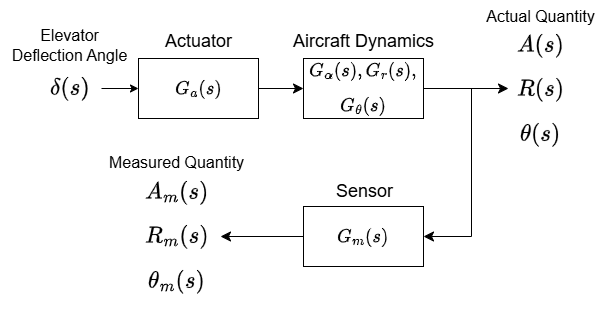
\includegraphics[width = \textwidth]{figs/ELE2038_H5_openLoopBlockDiagram.drawio.png}
            \caption{A block diagram of the open loop control system.}
            \label{fig:ol_blockDiagram}            
        \end{subfigure}%
        \begin{subfigure}[h]{0.5\textwidth}
            \centering
            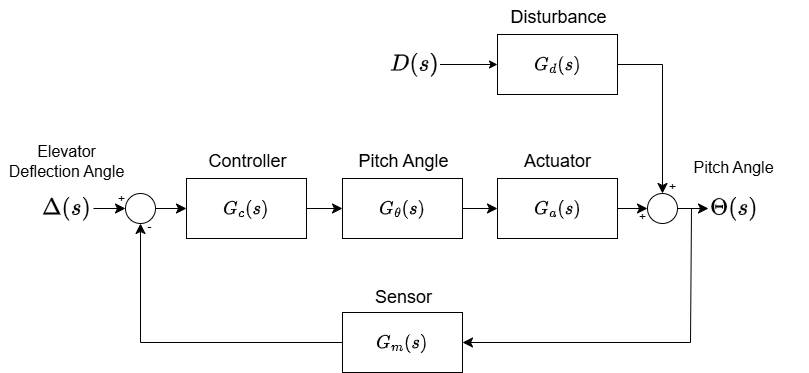
\includegraphics[width = \textwidth]{figs/ELE2038_H5_closedLoopBlockDiagram.drawio.png}
            \caption{A block diagram of the closed loop control system.}
            \label{fig:cl_blockDiagram}
        \end{subfigure}
    \caption{Block diagrams of the open and closed loop control systems.}
    \end{figure}
    
    \subsection{Analysis of $G_{\alpha}, G_{r}, G_{\theta}$.}
    From the system of differential equations the transfer functions of $G_{\alpha}$, $G_{r}$ and $G_{\theta}$ can be derived.
    \begin{subequations}
        \begin{align}
            G_\alpha =& \frac{0.232s + 1.26382}{(s + 0.31)(s + 0.425) + 0.9184} \\
            G_r =& \frac{0.0203s + 0.002581}{(s + 0.31)(s + 0.425) + 0.9184} \\
            G_\theta =& \frac{1.15101s + 0.1463427}{s((s + 0.31)(s + 0.425) + 0.9184)}
        \end{align}
    \end{subequations}
    The poles of $G_\alpha$ occur when $s^{2}+0.735s+1.05015=0$ which can be solved using the quadratic formula to give $s=-0.3675 \pm j0.9566$. The poles of $G_r$ also occur when $s^{2}+0.735s+1.05015=0$ and therefore result in the same value. Since $G_{\theta}(s)=\frac{56.7}{s}G_{r}(s)$; $G_{\theta}(s)$ shares all of the poles of $G_{r}(s)$, which are all stable, but also possesses an additional pole at $s=0$. This means the poles of $G_{\theta}(s)$ are $s=-0.3675 \pm j0.9566, s=0$. Since we have a pole with a non-negative real part, $G_{\theta}$ is not BIBO stable, meaning the open-loop system relating deflection angle of elevators to pitch angle is also not BIBO stable. This means a controller will be required to obtain BIBO stability of the system.
    \begin{figure}
    \centering
        \begin{subfigure}[h]{0.5\textwidth}
            \centering
            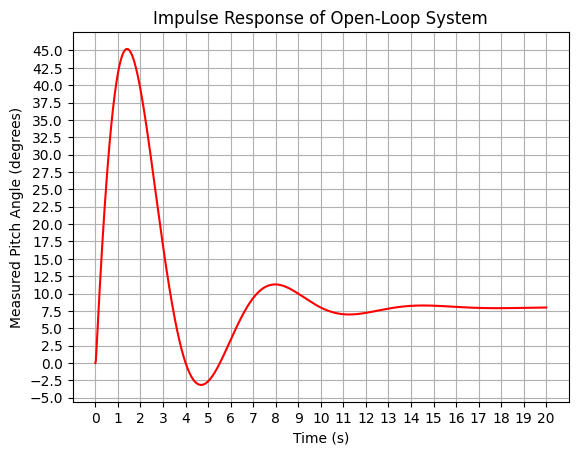
\includegraphics[width = \textwidth]{figs/GthetaImpRes.png}
            \caption{The impulse response of $G_\theta$.}
            \label{fig:gThetaImpRes}
        \end{subfigure}%
        \begin{subfigure}[h]{0.5\textwidth}
            \centering
            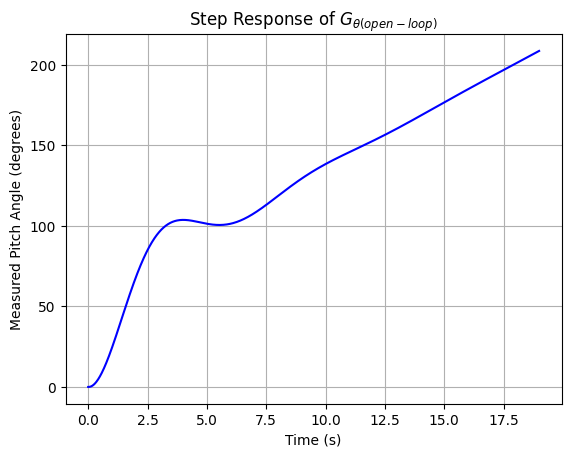
\includegraphics[width = \textwidth]{figs/GthetaStepRes.png}
            \caption{The step response of $G_\theta$.}
            \label{fig:gThetaStepRes}
        \end{subfigure}
    \caption{Output plots of $G_\theta$.}
    \end{figure}
    Figure \ref{fig:gThetaImpRes} shows that when the deflection angle of the elevators $\delta$ is a unit impulse, the pitch angle $\theta$ of the aircraft reaches a maximum of roughly 45 degrees after 1.5 seconds, before stabilising at (roughly) 7.5 degrees after around 16 seconds. Note that despite the input being a unit impulse, the pitch angle does not return to zero for the open-loop system.    Figure \ref{fig:gThetaStepRes} shows that as time increases, pitch angle $\theta$ is increasing unbounded. This follows from the prior discovery that $G_{\theta(\text{open-loop})}$ is not BIBO stable. The frequency response of $G_\theta$ is plotted along with the impulse, step and frequency responses of $G_\alpha$ and $G_r$ in the attached Python notebook.
    % ===============================
    \section{Testing Bode's Stability Criterion}
    We know that for a closed loop transfer function to be considered stable, it's corresponding open loop transfer function must meet the conditions outlined in Bode's Stability Criterion. If all conditions are met, then our closed loop system, $G_{cl}$, can be considered BIBO-stable. To verify the first criteria we find the poles of the open-loop system; in the Python notebook it has been shown that the poles all have a negative real part except for one that is at the origin. This satisfies the first criteria. In order to confirm the other criteria, a bode plot of the open-loop system has been plotted in the Python notebook, and from that we can conclude that there are crossover frequencies at $\omega_{\text{co,0}}=63, \; \omega_{\text{co,1}} = 630$, and $\omega_{\text{co,2}} = 1412$. This satisfies criteria 2 while further inspection of the graphs in the Python notebook reveal that $|G_{\text{ol}}(j\omega_{co,k})| < 1$ thus satisfying criteria 3. We can further stress test the system to find the gain and delay margins. In the Python notebook we have calculated that there is a gain margin of $29.5$ dB, delay margin of $0.15$ seconds and a phase margin of $21.6^\circ$. This indicates the system has adequate stability when faced with small time delays, although a larger delay margin would be favourable to make the system more stable.
    
    % ===============================
    \section{Disturbance Rejection}
    We will test our system with a disturbance input of $G_d = \frac{K}{\tau s + 1}$ where $K = \tau = 1$. The closed-loop system is shown in Figure \ref{fig:cl_blockDiagram}. The transfer function of the closed-loop system is thus given by
    \begin{equation}
        G_{L}(s) = \frac{G_d}{1 + G_c G_a G_\theta G_m}.
    \end{equation}
    Evaluating poles we find that there are two poles at the origin therefore meaning that the load trasfer function is not BIBO stable.
\end{document}